\begin{figure*}[ht]
\centering
\begin{lrbox}{\partiallisting}
\begin{minipage}{0.4\textwidth}
\begin{lstlisting}[basicstyle=\scriptsize\sffamily, stepnumber=1, numbers=left, numbersep=-6pt, framexleftmargin=0mm, framexrightmargin=0mm, language=Java, emph={allGames}]
    List<Game> allGames = gameMapper.getAllGamesByLeague(league);
    for (Game game : allGames) {
        game.getTeam1().setGame(game);
        game.getTeam2().setGame(game);
    }
    Collections.sort(allGames, new GameComparator());
\end{lstlisting}
\vspace{0.55cm}
\end{minipage}
\end{lrbox}
%\subcaptionbox{ABCD}{\usebox{\partiallisting}}
\usebox{\partiallisting}
\begin{lrbox}{\complisting}
\begin{minipage}{0.4\textwidth}
\begin{lstlisting}[basicstyle=\scriptsize\sffamily, stepnumber=1, numbers=left, numbersep=-6pt, framexleftmargin=0mm, framexrightmargin=0mm, language=java, emph={annotationVersion}]
    private boolean isValidUntil(Until annotation) {
        if (annotation != null) {
            double annotationVersion = annotation.value();
            if (annotationVersion <= version) {
                return false;
            }
        }
        return true;
    }
    \end{lstlisting}
\end{minipage}
\end{lrbox}
\usebox{\complisting}

\subcaptionbox{}[.45\textwidth]{
  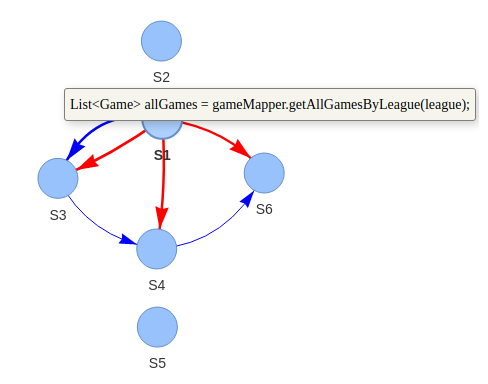
\includegraphics[width=0.8\linewidth]{icse23-demo-figures/lst-partial.png}
  \vspace{2cm}
}
\subcaptionbox{}[.45\textwidth]{
  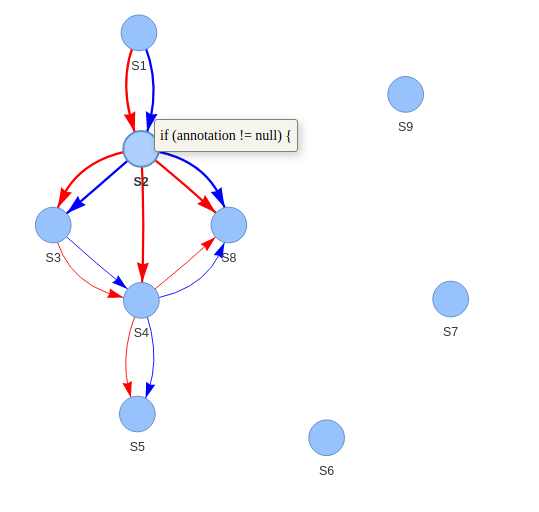
\includegraphics[width=\linewidth]{icse23-demo-figures/lst-complete.png}
}
\caption{Partial (top, left) and complete (top, right) Java code samples and their CFG/PDGs output by \tool (bottom).}
\label{fig:demo}
\end{figure*}